\documentclass[11pt,a4paper]{article}
\usepackage[margin=0.85in]{geometry}
\usepackage[T1]{fontenc}
\usepackage{lmodern}
\usepackage{amsmath,amssymb,mathtools}
\usepackage{graphicx,booktabs,array,enumitem}
\usepackage[dvipsnames]{xcolor}
\usepackage{microtype}
\usepackage{caption}
\usepackage{listings}
\usepackage{hyperref}
\hypersetup{colorlinks=true,linkcolor=MidnightBlue,urlcolor=MidnightBlue,
  pdfauthor={},pdfsubject={Reinforcement learning worked solutions}}
\setlength{\parindent}{0pt}
\setlength{\parskip}{6pt}
\setlist{nosep,leftmargin=*}
\setlength{\emergencystretch}{2em}
\captionsetup{font=small,labelfont=bf}
\lstset{basicstyle=\ttfamily\small,breaklines=true,
  columns=fullflexible,keepspaces=true,showstringspaces=false,
  commentstyle=\color{gray},keywordstyle=\color{MidnightBlue},
  aboveskip=6pt,belowskip=6pt}
\newcommand{\E}{\mathbb{E}}
\newcommand{\R}{\mathbb{R}}
\newcommand{\norm}[1]{\left\lVert #1\right\rVert}
\newcommand{\sg}{\operatorname{stopgrad}}
\DeclareMathOperator*{\argmax}{arg\,max}
\DeclareMathOperator*{\argmin}{arg\,min}
\newcommand{\studytitle}[1]{%
  \hypersetup{pdftitle={#1 - Worked Solutions}}%
  {\small\color{MidnightBlue} BASICRL\quad /\quad WORKED SOLUTIONS}\par
  \vspace{5pt}{\LARGE\bfseries #1}\par\vspace{5pt}}
\newcommand{\historical}{\textbf{Experiment status.} The following numbers and
  curves are retained from earlier runs, not from a rerun of the revised
  reference code. They are examples for interpretation, not performance guarantees.\par}

\begin{document}
\studytitle{Policy Gradients and Reward Shaping}

\section{The score-function identity}
Let $p_\theta(\tau)$ be a differentiable trajectory density on a support that
does not change locally with $\theta$. Assume that differentiation can pass
under the integral, for example by an integrable local dominating bound on
$\nabla_\theta p_\theta(\tau)R(\tau)$. The initial-state law, transition kernel,
and reward are independent of $\theta$. Then
\begin{align*}
 \nabla_\theta J(\theta)
 &=\int\nabla_\theta p_\theta(\tau)R(\tau)\,d\tau\\
 &=\int p_\theta(\tau)\nabla_\theta\log p_\theta(\tau)R(\tau)\,d\tau.
\end{align*}
The second step uses $\nabla p=p\nabla\log p$ wherever $p>0$.
Expanding the trajectory likelihood and differentiating its logarithm gives
\[
 \nabla_\theta\log p_\theta(\tau)
 =\sum_{t=0}^{H-1}\nabla_\theta\log\pi_\theta(a_t\mid s_t).
\]
The environment terms vanish because they have no explicit parameter dependence.
Random state visitation is still accounted for by the trajectory distribution.

\subsection{Causality, with the missing conditional step}
Let $\mathcal H_t$ contain the history through $s_t$, before sampling $a_t$,
and write $z_t=\nabla_\theta\log\pi_\theta(a_t\mid s_t)$. Conditional on that history,
\[
 \E[z_t\mid\mathcal H_t]
 =\int\nabla_\theta\pi_\theta(a\mid s_t)\,da
 =\nabla_\theta1=0.
\]
Past rewards are measurable with respect to $\mathcal H_t$. Therefore
\[
 \E\!\left[z_t\sum_{u<t}r_u\right]
 =\E\!\left[\left(\sum_{u<t}r_u\right)
                   \E[z_t\mid\mathcal H_t]\right]=0.
\]
With $G_t=\sum_{u=t}^{H-1}r_u$, this proves
\[
 \boxed{\nabla_\theta J=\E\!\left[\sum_{t=0}^{H-1}z_tG_t\right].}
\]

\subsection{Action-independent baselines}
For an integrable baseline $b_t(s_t)$ fixed during the actor update,
$\E[z_tb_t(s_t)\mid\mathcal H_t]=0$ by the same calculation. Conditioning
$G_t$ on $(s_t,a_t)$ yields the time-indexed $Q_t^\pi$, so
\[
 \nabla_\theta J=\E\!\left[\sum_tz_t\big(Q_t^\pi(s_t,a_t)-b_t(s_t)\big)\right].
\]
Choosing $b_t=V_t^\pi$ gives the true advantage. Use a detached baseline in
an autodifferentiated actor loss. A baseline fitted on the very same samples
can create additional statistical dependence; action independence is a
condition on the estimator, not merely on the network's input signature.

\newpage
\section{An undiscounted geometric-length example}
Let $K\geq0$ be the number of rewarded self-loops before the terminating
exit. For $0<\theta<1$,
\[
 \Pr(K=k)=(1-\theta)\theta^k,\quad R=k,\quad
 \frac{d}{d\theta}\log p_\theta(K=k)=\frac{k}{\theta}-\frac1{1-\theta}.
\]
This indexing includes immediate exit ($K=0$) and avoids confusing the number
of rewards with the total number of actions, which is $K+1$.

\subsection{Trajectory score calculation}
The geometric-series identities are
\[
 \sum_{k\geq0}k\theta^k=\frac{\theta}{(1-\theta)^2},\qquad
 \sum_{k\geq0}k^2\theta^k=\frac{\theta(1+\theta)}{(1-\theta)^3}.
\]
Consequently,
\begin{align*}
 J'(\theta)
 &=\sum_{k\geq0}(1-\theta)\theta^k
       \left(\frac{k}{\theta}-\frac1{1-\theta}\right)k\\
 &=\frac{1+\theta}{(1-\theta)^2}
          -\frac{\theta}{(1-\theta)^2}
 =\boxed{\frac1{(1-\theta)^2}}.
\end{align*}

\subsection{Direct return calculation}
Either sum the geometric distribution or condition on the first action:
\[
 J=\theta(1+J)+(1-\theta)0,\qquad
 J(\theta)=\frac{\theta}{1-\theta},\qquad
 J'(\theta)=\frac1{(1-\theta)^2}.
\]
At $\theta=1$, termination fails and the undiscounted return is infinite;
the formulas above are stated only for the interior parameter range.

\subsection{Reward-to-go calculation}
On a trajectory with $k$ self-loops, at loop $t=0,\ldots,k-1$ the score
is $1/\theta$ and the remaining reward is $k-t$. The exit has future reward 0.
Thus the sampled reward-to-go estimator is
\[
 g_{\rm RTG}(k)=\frac1\theta\sum_{t=0}^{k-1}(k-t)
             =\frac{k(k+1)}{2\theta}.
\]
Its expectation is
\begin{align*}
 \E[g_{\rm RTG}(K)]
 &=\frac{1-\theta}{2\theta}
   \left[\frac{\theta(1+\theta)}{(1-\theta)^3}
                 +\frac{\theta}{(1-\theta)^2}\right]
 =\frac1{(1-\theta)^2}.
\end{align*}
The estimators differ on individual trajectories but have the same mean.
Reward-to-go is a return estimator; it is not an advantage estimator unless
a suitable baseline has also been subtracted.

\newpage
\section{Potential-based reward shaping}
Assume $0<\gamma<1$, bounded rewards, and a fixed bounded potential $\Phi$.
For any policy $\rho$, not just the reference policy used to fit $\Phi$, define
$\widetilde r_t=r_t+\gamma\Phi(s_{t+1})-\Phi(s_t)$. The finite partial sum is
\begin{align*}
 \sum_{t=0}^{T-1}\gamma^t\widetilde r_t
 &=\sum_{t=0}^{T-1}\gamma^tr_t
   +\sum_{t=0}^{T-1}\big[\gamma^{t+1}\Phi(s_{t+1})-\gamma^t\Phi(s_t)\big]\\
 &=\sum_{t=0}^{T-1}\gamma^tr_t-\Phi(s_0)+\gamma^T\Phi(s_T).
\end{align*}
Since $|\gamma^T\Phi(s_T)|\leq\gamma^T\norm{\Phi}_\infty\to0$,
\[
 \boxed{\widetilde R=R-\Phi(s_0),\qquad
        \widetilde V^\rho(s)=V^\rho(s)-\Phi(s).}
\]
For each starting state, every policy's value is shifted by the same amount.
The set of maximizing policies is therefore unchanged. If $\widehat\pi$ is
an exact shaped optimum and $\pi^*$ an original optimum from every state,
\[
 \boxed{\norm{V^{\pi^*}-V^{\widehat\pi}}_\infty=0.}
\]
This does not imply $\widehat\pi=\pi^*$: multiple policies may have identical
optimal values. The estimate error $\norm{V^\pi-\widehat V}_\infty\leq\epsilon$
is not needed for policy invariance; boundedness of the fixed potential is
what makes the discounted boundary term vanish. The estimate may still
affect how easy the optimization problem is to learn.

\subsection{Episodic boundary conditions}
If a return is stopped at time $T$, the term $\gamma^T\Phi(s_T)$ remains.
Setting the terminal potential to zero removes it. Alternatively, continue
the process in an absorbing terminal state and include all subsequent
shaping rewards, which cancel the boundary term. Arbitrary nonzero terminal
potentials under stopped returns can change policy preferences.

\section{Importance-weighted off-policy gradients}
Let $\beta$ be a fixed behavior policy with $p_\theta\ll p_\beta$, and assume
the resulting integrand is absolutely integrable. Multiplying and dividing
by $p_\beta$ gives
\[
 \nabla_\theta J
 =\E_{\tau\sim p_\beta}\!\left[
       w_\theta(\tau)\nabla_\theta\log p_\theta(\tau)R(\tau)\right].
\]
The same initial distribution and dynamics cancel in the likelihood ratio:
\[
 \boxed{w_\theta(\tau)=\prod_{t=0}^{H-1}
                 \frac{\pi_\theta(a_t\mid s_t)}{\beta(a_t\mid s_t)},\qquad
 \nabla_\theta\log p_\theta(\tau)=\sum_{t=0}^{H-1}z_t.}
\]

\newpage
\subsection{What data reuse does and does not buy}
The identity permits estimating target-policy gradients from behavior data,
which is useful when new interactions are expensive. It requires support:
data from a behavior policy that never takes a needed action cannot recover
that action's contribution by weighting. Products of likelihood ratios may
have very high or even infinite variance as the horizon or policy mismatch
increases. Clipping and self-normalizing weights generally introduce
finite-sample bias. Data reuse does not guarantee improved effective sample size.

For a score-function surrogate, treat a computed importance weight as fixed
when multiplying it by a log probability. Differentiating both factors in
$-w_\theta\log p_\theta R$ adds an unwanted term. Directly differentiating
$-w_\theta R$ is a different valid construction when its conditions hold.

\section{The discounted programming objective}
The notebook uses $J_\gamma=\E[\sum_{u=0}^{H-1}\gamma^ur_u]$. Causality gives
\[
 \nabla J_\gamma
 =\E\!\left[\sum_{t=0}^{H-1}\gamma^t z_tG_t^\gamma\right],\qquad
 G_t^\gamma=\sum_{u=t}^{H-1}\gamma^{u-t}r_u.
\]
The relative discount inside $G_t^\gamma$ does not replace the outer
$\gamma^t$. For vanilla REINFORCE, multiply each score by the same full
discounted return. For reward-to-go, use $\gamma^tG_t^\gamma$ as its weight.
\begin{lstlisting}
returns = torch.empty_like(rewards)
running = rewards.new_zeros(())
for t in reversed(range(len(rewards))):
    running = rewards[t] + gamma * running
    returns[t] = running
discounts = gamma ** torch.arange(len(rewards), device=rewards.device)
weights = discounts * returns if reward_to_go else returns[0]
log_prob = policy(states).log_prob(actions).sum(-1)
loss = -(log_prob * weights.detach()).sum()
\end{lstlisting}
Average these per-trajectory losses over trajectories. Summing log densities
over the action dimension forms the joint density of independent action
coordinates. Relative discounts, episode length, and batch normalization
must match the objective being compared.

A Gaussian is a continuous \emph{density}, which may exceed one; its log
density may be positive. Thus the sign of the policy loss does not tell
whether the agent performs well. Evaluate actual episode return and success,
and use repeated seeds to measure variability.

\newpage
\section{Retained learning curves}
\historical
\begin{figure}[!ht]
 \centering
 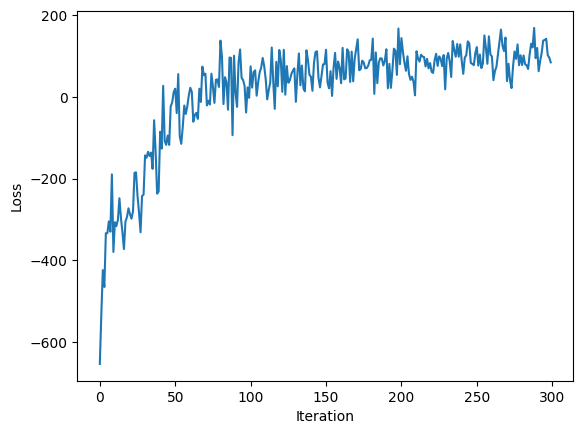
\includegraphics[width=0.62\linewidth]{figures/reinforce-loss.png}
 \par\vspace{8pt}
 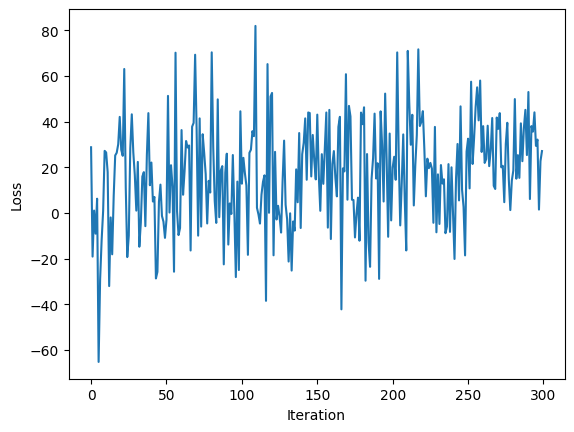
\includegraphics[width=0.62\linewidth]{figures/reward-to-go-loss.png}
 \caption{Historical surrogate losses: vanilla REINFORCE (top) and
 reward-to-go (bottom). Their signs and trends do not measure policy quality.
 The revised implementation includes the outer discount factor; these old
 curves do not validate that revision.}
\end{figure}

\textbf{Solution scope.} The gradient equalities hold under the stated
differentiability, integrability, support, and environment-independence
conditions. Shaping preserves the set of optimal policies under the stated
boundary conditions. No empirical variance reduction is established solely
by comparing these two surrogate-loss plots.
\end{document}
